% !TeX spellcheck = en_US
\documentclass[letterpaper,12pt,twoside]{report}
\usepackage{fancyhdr}
\usepackage{fullpage}
\usepackage{tikz}

\begin{document}
	\pagestyle{fancy}
	\fancyhf{}
	\fancyhead[L]{Day ???}
	\fancyhead[R]{\textit{The Calendar Project}}
	\fancyfoot[L]{Citations Involved: 1, 2, 3}
	
	% Problem
	\textbf{Problem}
	\begin{quote}
	\textsf{When all the diagonals in a regular hexagon are drawn, how many pairs of diagonals will be perpendicular?}
	\end{quote}
	
	% Graphics
	\begin{center}
		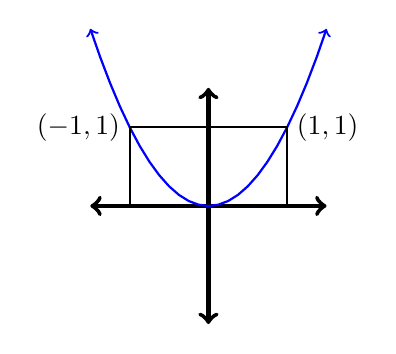
\begin{tikzpicture}
		\draw [<->][ultra thick] (-1.5,0) -- (1.5,0);
		\draw [<->][ultra thick] (0,1.5) -- (0,-1.5);
		
		\draw [<->][blue, thick, domain=-1.5:1.5] plot (\x, {\x*\x});
		\draw [thick] (-1,0) -- (-1, 1) -- (1, 1) -- (1, 0);
		
		\node[left] at (-1,1) {$(-1,1)$};
		\node[right] at (1,1) {$(1,1)$};
		
		\end{tikzpicture}
	\end{center}
	
	% Reasoning
	\begin{minipage}[t]{.6\textwidth}
		\textbf{Reasoning}
		
		
	\end{minipage}
	\begin{minipage}[t]{.4\textwidth}
		\textbf{External References}
		
		
	\end{minipage}

\end{document}